\documentclass[12pt]{article}

%Paquetes
\usepackage[left=2cm,right=2cm,top=3cm,bottom=3cm,letterpaper]{geometry}
\usepackage{lmodern}
\usepackage[T1]{fontenc}
\usepackage[utf8]{inputenc}
\usepackage[spanish,activeacute]{babel}
\usepackage{mathtools}
\usepackage{amssymb}
\usepackage{enumerate}
\usepackage{tabularx}
\usepackage{wasysym}
\usepackage{listings}
\usepackage{graphicx}
\usepackage{hyperref}
%\usepackage{graphicx}
%\graphicspath { {tarea01/media/} }
%\usepackage{pifont}
\usepackage{listings}

%Preambulo
\title{Tecnologías para desarrollos en internet \\ Manual CRUD: Beego}
\author{Kihui-DEV}
\date{Fecha: 18/09/16 \\ Facultad de Ciencias UNAM}

\begin{document}
\maketitle
\tableofcontents{}
\newpage

\section{Introducción}
Hola
\newpage
\section{Instalación de Go 1.7}
Paquetes de instalación para \textit{Apple OS X, Microsoft Windows y Linux} son provistos en la página oficial de descargas de \href{https://golang.org/dl/}{Go}. También viene incluido entre las opciones el código fuente del compilador del lenguaje junto con instrucciones para llegar a una instalación tan completa como las demás. \par
A continuación, presentamos la instalación para \textit{Linux y OS X}. \footnote{Si se desea revisar la configuración para \textit{Windows}, hacer uso del siguiente enlace:
  \href{https://golang.org/doc/install?download=go1.7.1.windows-amd64.msi}{MSI Installer}}

\subsection{Descarga}\label{sec:d}


\subsubsection*{Linux}
Para obtener el paquete de Golang\footnote{Actualmente la versión 1.7.1} \\
Ejecutar:
\begin{verbatim}
  $ wget https://golang.org/doc/install?download=go1.7.1.linux-amd64.tar.gz
\end{verbatim}
O bien descargarlo directamente desde este enlace:
\begin{center}
\href{https://golang.org/doc/install?download=go1.7.1.linux-amd64.tar.gz}{Go 1.7 para Linux y OS X}.
\end{center}


\subsubsection*{Mac OS X}
Alternativa a las siguientes instrucciones, existe la opción de descargar el fichero \textit{.pkg} instalable de \textit{Go} que automatiza la configuración para este sistema operativo.\footnote{\href{https://golang.org/doc/install?download=go1.7.1.darwin-amd64.pkg}{Instalador para Mac OS X}}\\[1mm]

Para obtener una configuración inicial personalizada \textit{Mac OS X} utilice el paquete descargable para \textit{Linux} disponible en la sección anterior.\\

El resto de la configuración se sigue de la misma manera para ambas plataformas.

\subsection{Configuración}\label{sec:c}
Primero extraemos los archivos del paquete comprimido sobre algún directorio.\\
Para descomprimir el paquete sobre \textit{/usr/local} como es usual:
\begin{verbatim}
  # tar -C /usr/local -xzf go1.7.1.linux-amd64.tar.gz
\end{verbatim}
Al finalizar la extracción, procedemos a establecer una ruta a los binarios de las herramientas de \textit{Go}, y así tenerlas disponibles en cada sesión.\par
Agregar esta línea en el script de inicio (típicamente sobre \textit{/user/local/profile}
si se desea hacer una instalación general en el sistema operativo o
en particular para el usuario en curso, usar en cambio \textit{\char126/.profile}):
\begin{verbatim}
  export PATH=$PATH:/usr/local/go/bin
\end{verbatim}

\subsection{Prueba}
Crear un directorio que haga de workspace para la prueba.\\
Por ejemplo:
\begin{verbatim}
  $ mkdir ~/go
\end{verbatim}
Asignar la variable \textbf{GOPATH}\footnote{La misma línea puede agregarse al script de inicio \textit{profile} manejado en la sección de configuracion para evitar ejecutarla y mantener los proyectos y aplicaciones de \textit{Go} ubicados en un sólo directorio.}
para que apunte a tal dirección:
\begin{verbatim}
  $ export GOPATH=$HOME/go
\end{verbatim}
Bien podemos hacer persistente este cambio agregando la misma línea al script
de inicio que editamos en la sección anterior (ir a Descarga~\ref{sec:d} y configuración~\ref{sec:c}). \par

A continuación, creamos dentro de ese directorio  \textit{src/hola}.
Y dentro de \textit{hola/} un fichero nuevo de nombre \textit{hola.go}:
\begin{verbatim}
     package main

     import "fmt"

     func main() {
         fmt.Printf("hola, mundo\n")
     }
\end{verbatim}

Luego, desde cualquier ubicación podemos ejecutar\\
esto:
\begin{verbatim}
  $ go install hola
\end{verbatim}

Esto producirá un ejecutable \textit{hola} dentro de el directorio \textit{go/bin/},
que podemos ejecutar utilizando lo siguiente:
\begin{verbatim}
  $ $GOPATH/bin/hola
\end{verbatim}

o directamente sobre el directorio donde se encuentre el ejecutable:

\begin{verbatim}
  $ ./hola
\end{verbatim}

Si produce la salida ``hola, mundo'', quiere decir que nuestra instalación fue exitosa. \newpage


\section{Instalación de Beego}

\noindent Para instalar la última versión de Beego\footnote{A la fecha de elaboración de este manual: 1.7.1} utilizamos el siguiente comando:
\begin{verbatim}
  $ go get github.com/astaxie/beego
\end{verbatim}

\noindent Para compilar y correr nuestros proyectos necesitaremos instalar Bee\footnote{A la fecha de elaboración de este manual: 1.5.2} también :
\begin{verbatim}
  $ go get github.com/beego/bee
  $ go install github.com/beego/bee
\end{verbatim}

Para poder utilizar \textit{bee} sin necesidad de ir a la carpeta de binarios de \textit{Go}, podemos crear un enlace simbólico que apunte precisamente al ejecutable.
\begin{verbatim}
  # ln -s $GOPATH/bin/bee /usr/bin/bee
\end{verbatim}

\section{Creación de proyecto}\label{sec:proy}
\noindent Para crear un proyecto en Beego, necesitamos ir al directorio de nuestro $\$$GOPATH, donde escribimos el siguiente comando:
\begin{verbatim}
$ bee new beego-crud
\end{verbatim}
\noindent Podremos ver que se han creado las siguientes carpetas y archivos necesarios para nuestra aplicación:

\begin{verbatim}
beego-crud/
|-- conf/
|   |__ app.conf
|-- controllers/
|   |__ default.go
|-- main.go
|-- models/
|-- routers/
|   |__ router.go
|-- static/
|   |--- css/
|   |--- img/
|   |___ js/
|-- tests/
|   |__ default_test.go
|-- views/
    |__ index.tpl
\end{verbatim}

\subsection{Estructura del proyecto - MVC}
\begin{enumerate}[1)]
  \subsubsection*{Modelo}
\item \textit{conf/}
\item \textit{models/}
  \subsubsection*{Vista}
\item \textit{views/}
  \subsubsection*{Controlador}
\item \textit{controllers/}
\item \textit{routers/}
  \subsubsection*{Extra}
\item \textit{static/}
\item \textit{tests/}

\end{enumerate}


\subsection{Prueba del servidor local}
\noindent Finalmente para correr el nuevo proyecto que hemos creado, hacemos lo siguiente:
\begin{verbatim}
$ cd $GOPATH/src/beego-crud
$ bee run
\end{verbatim}
\noindent Ingresamos \textit{localhost:8080} como dirección en el navegador para encontrarnos con la siguiente página de inicio: \\

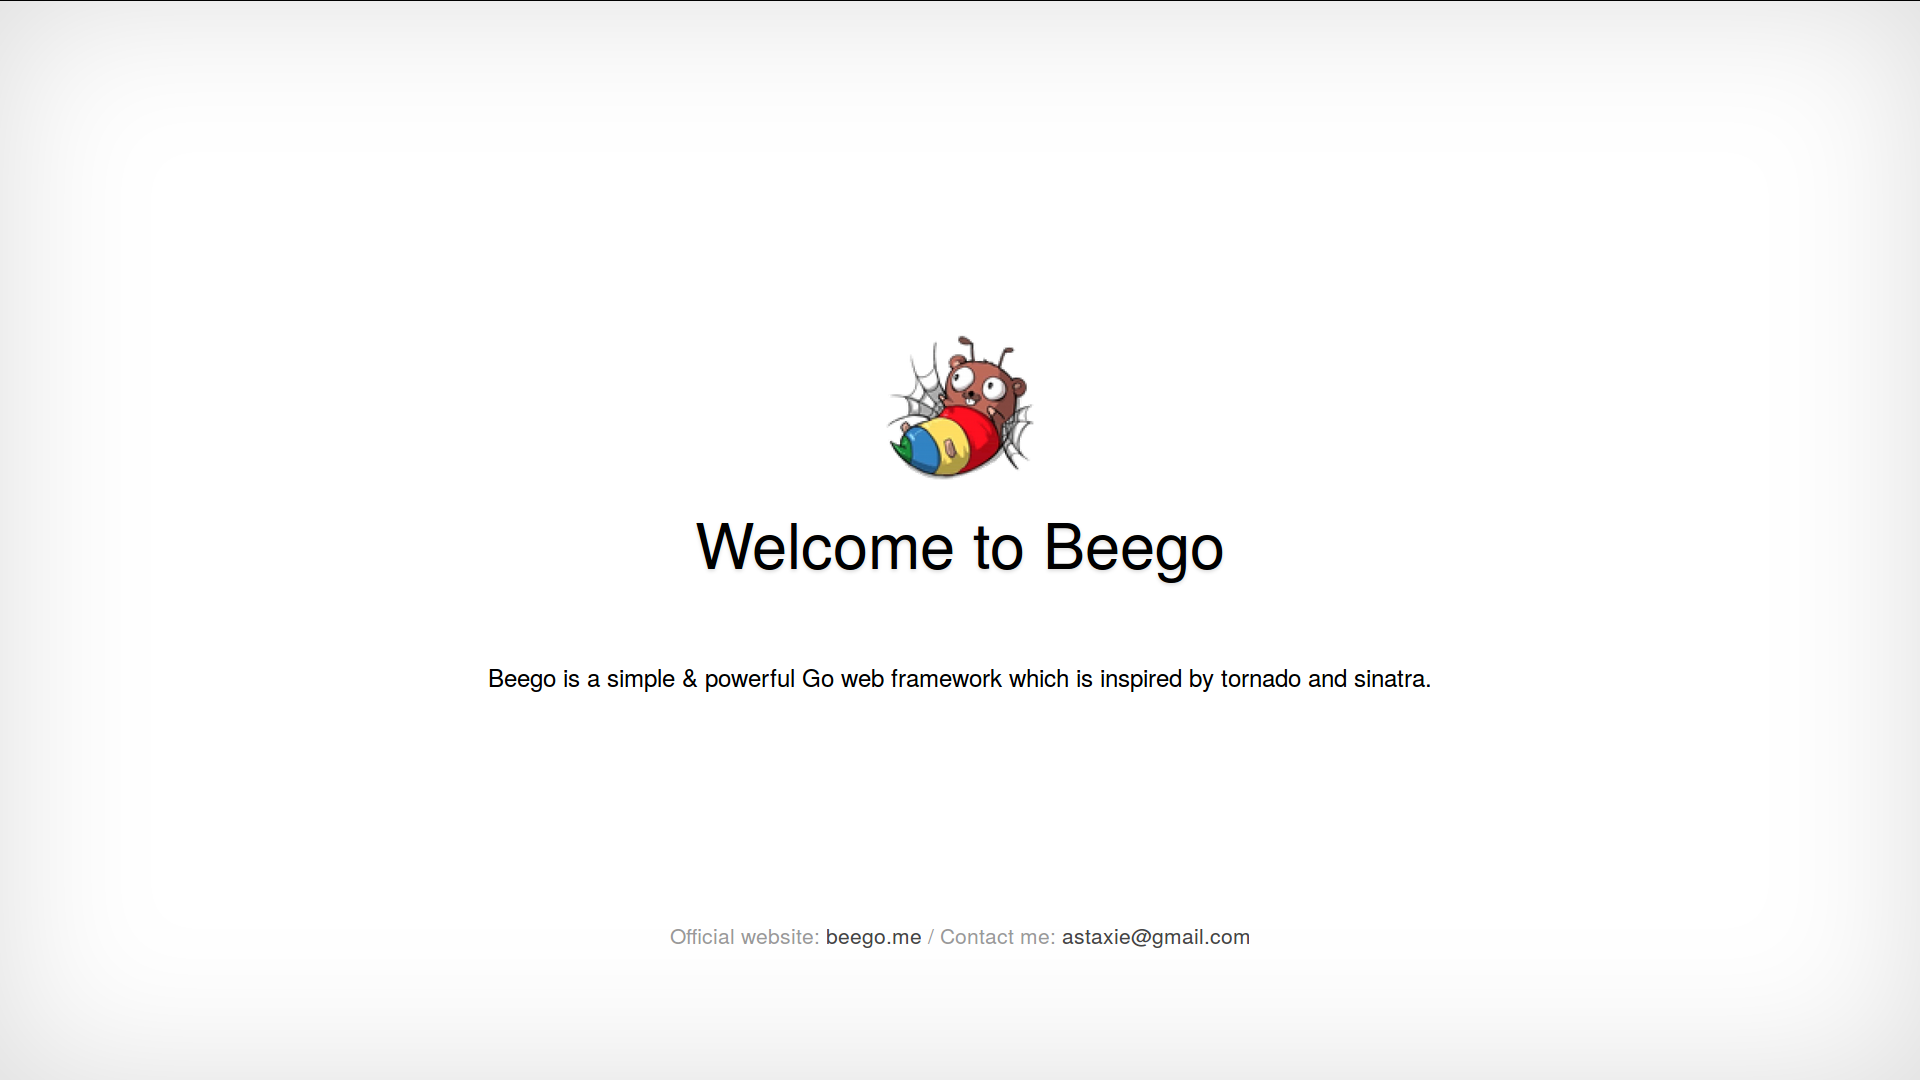
\includegraphics[scale=0.25]{beego.png}
\newpage

\section{Elaboración del CRUD bajo MVC}
En esta sección revisaremos la implementación de un CRUD (\textit{Create-Read-Update-Delete}) sobre la aplicación que creamos en la sección anterior (s.~\ref{sec:proy}). Comenzaremos explicando los documentos que tenemos que modificar para tener una configuración exitosa y la forma de escribir el código de acuerdo al MVC (\textit{Modelo Vista Controlador}), siguiendo la estructura que nos proporciona \textit{Beego} para éste.

\subsection{Preparación}
%Para implementar nuestro primer CRUD en Beego es necesario tener un sistema de
%datos persistente sobre el
%que realicemos nuestras operaciones.
%La mejor solución que en casi todos los casos se señala para lograr esto en el desarrollo
%web por supuesto no son los archivos, sino una base de datos, por lo general
%relacional. \par
Todo proyecto de Beego, como ya vimos, está organizado segun el MVC. Es precisamente
sobre el archivo de \textbf{models.go} que escribiremos nuestras
relaciones expresadas con atributos asignados de acuerdo a los tipos de dato
que maneja Go para después verlos reflejados en tablas en una base datos ya explorable.
Bien podría ser en sentido inverso, desde un esquema \textit{SQL} generar los modelos
para nuestro proyecto de Beego, pero en nuestro caso decidimos implementarlo
en esta dirección porque nuestra intención es enfocarnos en Beego, no en SQL.\par
A continuación presentamos la configuración de la base de datos y un mapeo
de una sola relación con la que trabajaremos todas las operaciones.
\subsubsection*{Base de datos}
\textit{Beego-ORM} es la herramienta de Mapeo Objeto-Relacional de \textit{Beego}
escrita en \textit{Go}. Según la página oficial está inspirada en \textit{Django ORM}
y \textit{SQLAlchemy}. Se advierte que al estar en desarrollo, no se garantiza
un 100\% de compatibilidad y es posible encontrar algunos ``bugs'', que el
equipo de desarrollo de Beego promete solucionar apenas se reporten.\\

Lo primero que hay que considerar es la conexión con la base de datos que necesitamos para nuestro modelo.
Beego provee soporte para tres sistemas manejadores de bases de datos
con sus respectivos ``drivers'':
\begin{itemize}
\item \href{http://www.mysql.com/}{MySQL}
\item \href{https://sqlite.org/}{Sqlite}
\item \href{http://www.postgresql.org.es/}{Postgres}
\end{itemize}

Por su sencilla configuración y mayoría de ejemplos de implementación junto con
Beego, escogimos MySQL por lo que los siguientes puntos se ejemplificarán
con el supuesto de que trabajamos con este SMBD\footnote{Para revisar más ampliamente
  las opciones de bases de datos recomendamos visitar este apartado de la documentación:
  \href{http://beego.me/docs/mvc/model/orm.md\#set-up-database}{ORM Usage}} y que ya se cuenta con una instalación
funcional\footnote{En el manual de MySQL v5.7 viene una amplia guía de instalación.
  Recomendamos los siguientes apartados para distintos sistemas operativos:
  \href{http://dev.mysql.com/doc/refman/5.7/en/windows-installation.html}{Windows} |
  \href{http://dev.mysql.com/doc/refman/5.7/en/osx-installation.html}{OS X} |
  \href{http://dev.mysql.com/doc/refman/5.7/en/linux-installation.html}{Linux}}.\\[2mm]
Lo primero que haremos será crear nuestra base de datos:
\begin{verbatim}
  $ mysql -u root -p
  MariaDB [(none)]> create database beego;
  MariaDB [(none)]> exit
\end{verbatim}
Si no experimentamos ninguna dificultad con esto, podemos continuar con la
configuración de nuestro proyecto.
\subsubsection*{Configuración}
Todo proyecto de \textit{Beego} cuenta con un archivo de configuración.
Por defecto se interpreta el archivo \textbf{app.conf} bajo el directorio
\textit{conf/} de la aplicación. Inicialmente, dicho archivo está escrito en formato INI
\footnote{También se permiten los siguientes formatos: XML, JSON y YAML},
una sintáxis sencilla, compuesta de
secciones, propiedades y valores sobre archivos de texto plano. Por ejemplo, en ella podremos escribir
configuraciones del estilo:
\begin{verbatim}
  [seccion]
  nombre_propiedad = valor
\end{verbatim}

Nosotros conservaremos el nombre de la aplicación (appname), el puerto http
(httport) y el modo de ejecución (runmode); propiedades que ya vienen incluídas
al momento de creación de nuestra nueva aplicación. Adicionalmente
escribiremos las siguientes propiedades:\footnote{El caracter ``;'' denota una línea de comentario. No es necesario
  al final de cada línea. }
\begin{verbatim}
  mysqluser = "root" ;el nombre del usuario de MySQL que es dueño de la base
  mysqlpass = "magdario" ;la contraseña de acceso del usuario MySQL
  mysqldb = "beego" ;el nombre de la base de datos que creamos anteriormente
  mysqlurls = "127.0.0.1" ;la dirección del host de la base de datos (localhost)
\end{verbatim}

Gracias a esta configuración la aplicación podrá establecer
conexión con nuestra base de datos para llevar a cabo las operaciones.

\subsubsection*{Modelos}\label{sec:p}
Como ya señalamos previamente, para realizar el CRUD, nos auxiliaremos de una
sola relación en la base de datos.
Para registrarla, basta definir una estructura
sobre el archivo de Go \textbf{models.go}, ubicado en la carpeta \textit{models/}
de nuestra aplicación. Aquí mostramos un ejemplo de cómo podría ser un modelo de
usuario\footnote{Para revisar con más detenimiento el código, pruebe visualizar
  el archivo del proyecto en GitHub: \href{https://github.com/Kihui/Beego-CRUD/blob/master/models/models.go}{models.go}}:

\begin{verbatim}
  type Usuario struct {
      Id          int
      Nombre      string
      Edad        int
  }
\end{verbatim}


Para continuar con el mapeo y ver nuestro nuevo modelo reflejado en la base
de datos que configuramos previamente,
ahora nos dirigimos al archivo \textbf{main.go} en la raíz del proyecto y
agregamos las siguientes configuraciones a los ``imports'' del programa:
\begin{verbatim}
    "github.com/astaxie/beego/orm"
    _ "github.com/go-sql-driver/mysql"
    models "beego-crud/models"
\end{verbatim}
Esto con el fin de que podamos utilizar Beego-ORM, el driver del SMBD
y los modelos que declaremos. \\
Luego, creamos un nuevo método método \textit{init()}, en el que escribiremos:
\begin{verbatim}
    func init() {
        orm.RegisterDriver("mysql", orm.DRMySQL)
        orm.RegisterDataBase("default", "mysql", "root:magdario@/beego?charset=utf8")
        orm.RegisterModel(new(models.Usuario))
        orm.RunCommand()
    }
\end{verbatim}

Con esto, registramos tanto el driver que utilizaremos como la base de datos sobre
la que se realizaran las operaciones de los modelos que ``demos de alta''
en este método. Es importante señalar que si no registramos los modelos aquí o
en su archivo correspondiente, no serán ``visibles'' para nuestra aplicación y no
será posible efectuar cambios sobre ellos. Nosotros elegimos registrar el modelo
de \textit{usuario}  en el método de inicialización, por la forma explícita que nos provee. \\

\noindent
Recomendamos revisar la forma resultante del archivo: \href{https://github.com/Kihui/Beego-CRUD/blob/master/main.go}{main.go} \\

Finalmente, compilamos \textbf{main.go} y lo ejecutamos con los parámetros necesarios
para realizar el mapeo y la sincronización con la base de datos.\\

\noindent
Desde \textit{\$GOPATH/beego-crud} ejecutamos:
\begin{verbatim}
  $ go build main.go
  $ ./main orm syncdb
\end{verbatim}

\noindent
Para revisar que todo marcha bien podemos pedirle al ``prompt'' de MySQL que nos
muestre las tablas de nuestra base de datos:
\begin{verbatim}
  MariaDB [(none)]> use beego;
  MariaDB [beego]> show tables;
\end{verbatim}

\noindent
Que debe resultarnos en algo similar a:
\begin{verbatim}
+-----------------+
| Tables_in_beego |
+-----------------+
| usuario         |
+-----------------+
\end{verbatim}

Si en efecto nos encontramos con las tablas correspondientes a los modelos que
registramos, ya podemos dedicarnos a escribir el controlador y las vistas
pertinentes para nuestro CRUD, sin preocuparnos por la conexión con la base
de datos.\\

A continuación presentamos las operaciones de un CRUD implementado en nuestro
Framework Beego. Cada una viene separada con su sección correspondiente y los
apartados que contiene se refieren a los archivos de la estructura del proyecto
y cómo debemos modificarlos para elaborar la operación en cuestión.\\

\subsection{Creación}
Manejaremos esta operación como un registro de usuarios para alguna plataforma.
Este registro será lo primero que tendremos en el ``index'' de la página que
estamos desarrollando.
\subsubsection{Controllers}
Lo primero que debemos considerar es la función del controlador que manejara
nuestra operación de creación. En el archivo controllers/\textbf{default.go}\footnote{Podemos cambiar este nombre de archivo si nos parece pertinente, pero por simplicidad lo dejaremos así, basta con que nuestras funciones de controlador se ubiquen en esa carpeta.}
encontraremos la estructura del controlador principal, sus métodos serán los que
manejen las respuestas del servidor ante las peticiones de la interfaz.
Antes de comenzar con nuestra función de agregado o creación de usuario, importaremos
los modelos de la aplicación que ya hemos considerado\footnote{Preparación - Modelos \ref{sec:p}},
la herramienta \textit{ORM}, una herramienta de validación de datos y la herramienta estándar de Go
\textit{fmt}:
\begin{verbatim}
    import (
      "github.com/astaxie/beego"
      models "beego-crud/models"
      "github.com/astaxie/beego/orm"
      "github.com/astaxie/beego/validation"
      "fmt"

    )
\end{verbatim}
\begin{lstlisting}[language=go]
\end{lstlisting}
\subsubsection{Routers}
En la estructura \textit{MainController} a la
que se hace referencia \textit{init()} del archivo routers/\textbf{routers.go} que nos
proporciona Beego por defecto en todo nuevo proyecto:
\begin{verbatim}
     beego.Router("/", &controllers.MainController{})
\end{verbatim}
Ahora, modificaremos esa línea para que sea acorde a nuestra operación de creación.
\subsubsection{Views}
\href{https://github.com/Kihui/Beego-CRUD/blob/master/controllers/default.go\#L29}{Add()}
\subsection{Lectura}
\subsubsection{Controllers}
\subsubsection{Routers}
\subsubsection{Views}
\href{https://github.com/Kihui/Beego-CRUD/blob/master/controllers/default.go\#L15}{View()}
\subsection{Actualización}
\subsubsection{Controllers}
\subsubsection{Routers}
\subsubsection{Views}
\href{https://github.com/Kihui/Beego-CRUD/blob/master/controllers/default.go\#L94}{Update()}
\subsection{Eliminación}
\subsubsection{Controllers}
\subsubsection{Routers}
\subsubsection{Views}
\href{https://github.com/Kihui/Beego-CRUD/blob/master/controllers/default.go\#L64}{Delete()}

\subsection{Resultados}
Nota: agregar screenshots de la aplicación web
\section{Referencias}
Nota: agregar formato!\\
\noindent
\url{http://beego.me/docs/intro} \\
\url{https://golang.org/}\\
\url{https://www.mysql.com/} \\
\url{http://wiki.freepascal.org/Using_INI_Files} \\
\url{http://dspace.howest.be/bitstream/10046/1323/1/anton-van-eechaute-2016-03-25.pdf}
\end{document}
